\section{Static responses of the structure}
\label{sec:static_responses}

In this section, the static responses of the structure are computed.
The static responses are the displacements of the structure when subjected to a static load.

Again, as in many other engineering problems, we can approach this problem in at least a couple of different ways.
In the following, we will explain how to compute the static responses of the structure using both a displacement approach and an acceleration approach.

Notice that the two method differs only in the way the global force vector $\mathbf{F}$ is assembled.
In the end, once $\mathbf{F}$ is known, both methods will solve the steady state version of the equation of motion:

\begin{equation}
    \mathbf{K} \mathbf{u} = \mathbf{F}
    \label{eq:static_responses}
\end{equation}

Where $\mathbf{K}$ is the stiffness matrix of the structure, $\mathbf{u}$ is the vector of displacements and $\mathbf{F}$ is the global force vector.

\subsection{Displacement approach}
\label{subsec:displacement_approach}

The displacement approach consists of assembling the global force vector $\mathbf{F_F}$ based on the `displacement method' used in structural mechanics.

In particular, if the structure is subjected to a distributed static load (as in the case of the gravity load), we know that the nodal forces on a single beam element can be computed as:

\begin{figure}[H]
    \centering
    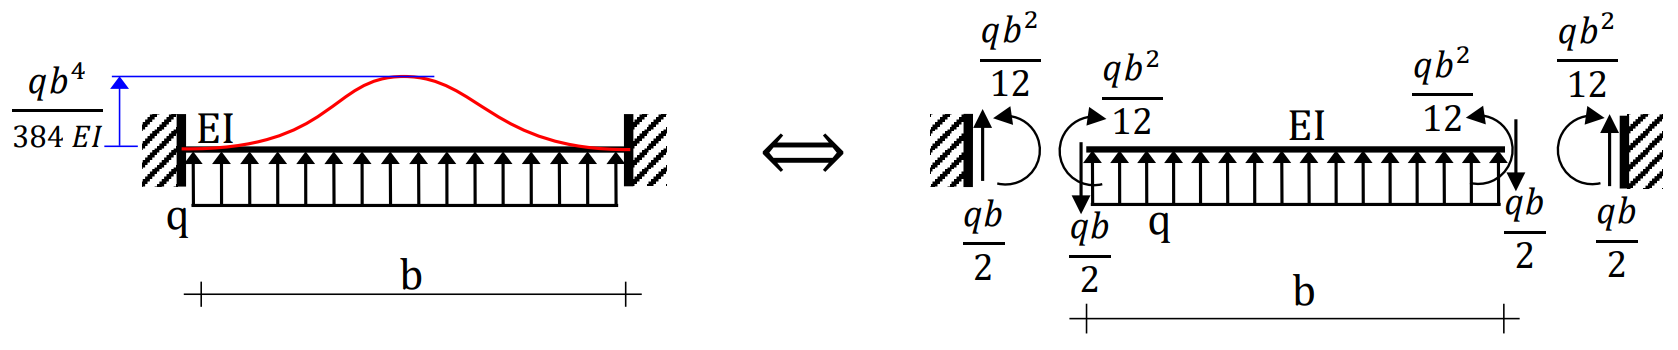
\includegraphics[width=0.9\textwidth]{img/displacement-method.png}
    \caption{Displacement method for distributed loads.}
    \label{fig:displacement_method}
\end{figure}

From the figure above, we can obtain the coefficients needed to compute the equivalent nodal forces due to a distributed load along the element.

By using proper change in the reference system (by rotational matrices), it's possible to build the equivalent global force vector $\mathbf{F_F}$, which can be seen as the equivalent effect on the node of the structure due to the distributed load.

Finally, we can solve the equation of motion \ref{eq:static_responses} to obtain the displacements of the structure.

In \texttt{MATLAB}, the displacement approach can be implemented as follows:

\begin{lstlisting}[language=Matlab, caption={Displacement approach to compute the static responses of the structure.}]
    % Displacement approach.
    F_F_global = zeros(3*nnod, 1);

    for ii = 1:nbeam

        [R, Q] = compute_rotational_matrices(gamma(ii));

        % Here we are negletting the possibility of a distributed momentum
        % load. Just distributed force loads are considered.
        elemental_distributed_load = R(1:2, 1:2)' * [0 -9.81 * m(ii)]';

        elemental_equivalent_nodal_load = [
            l(ii)/2 0
            0       l(ii)/2
            0       l(ii)^2/12
            l(ii)/2 0
            0       l(ii)/2
            0       -l(ii)^2/12
            ] * elemental_distributed_load;

        global_equivalent_nodal_load = Q * elemental_equivalent_nodal_load;

        F_F_global(incid(ii, :)) = F_F_global(incid(ii, :)) + global_equivalent_nodal_load;

    end

    X_gravity_displacement_approach = K_FF \ F_F_global(1:ndof);
\end{lstlisting}
\subsection{Acceleration approach}
\label{subsec:acceleration_approach}

The acceleration approach instead, consists of assembling the global force vector $\mathbf{F_F}$ based on the idea that the structure (since it has been discretized), can be seen as a system of masses connected by springs and dampers.
Because of this, a distributed acceleration load can be directly transformed into a series of nodal forces by solving the second Newton's law for each node of the structure.

In particular, the nodal forces can be computed as:

\begin{equation}
    \mathbf{F_F} = [M_{FF}] \cdot \mathbf{a}
\end{equation}

Where $[M_{FF}]$ is the mass matrix of the structure and $\mathbf{a}$ is the vector of accelerations acting on each degree of freedom of the structure.

Finally, we can solve the equation of motion \ref{eq:static_responses} to obtain the displacements of the structure.

In \texttt{MATLAB}, the acceleration approach can be implemented as follows:

\begin{lstlisting}[language=Matlab, caption={Acceleration approach to compute the static responses of the structure.}]
    % Acceleration approach.
    x_dot_dot = zeros(ndof, 1);
    x_dot_dot(idb(:, 2)) = -9.81;

    F_F_nodal = M * x_dot_dot;

    X_gravity_acceleration_approach = K_FF \ F_F_nodal(1:ndof);
\end{lstlisting}

\subsection{Comparison of the two methods}
\label{subsec:comparison_of_the_two_methods}

As we can see from Figure \ref{fig:static_responses}, the two methods give the same results.
This is expected given that the acceleration approach is just a derivation of the displacement approach, since the mass matrices $M$ and the stiffness matrices $K$ are just an implementation of the displacement and/or the force method used to solve structures.

\begin{figure}[H]
    \centering
    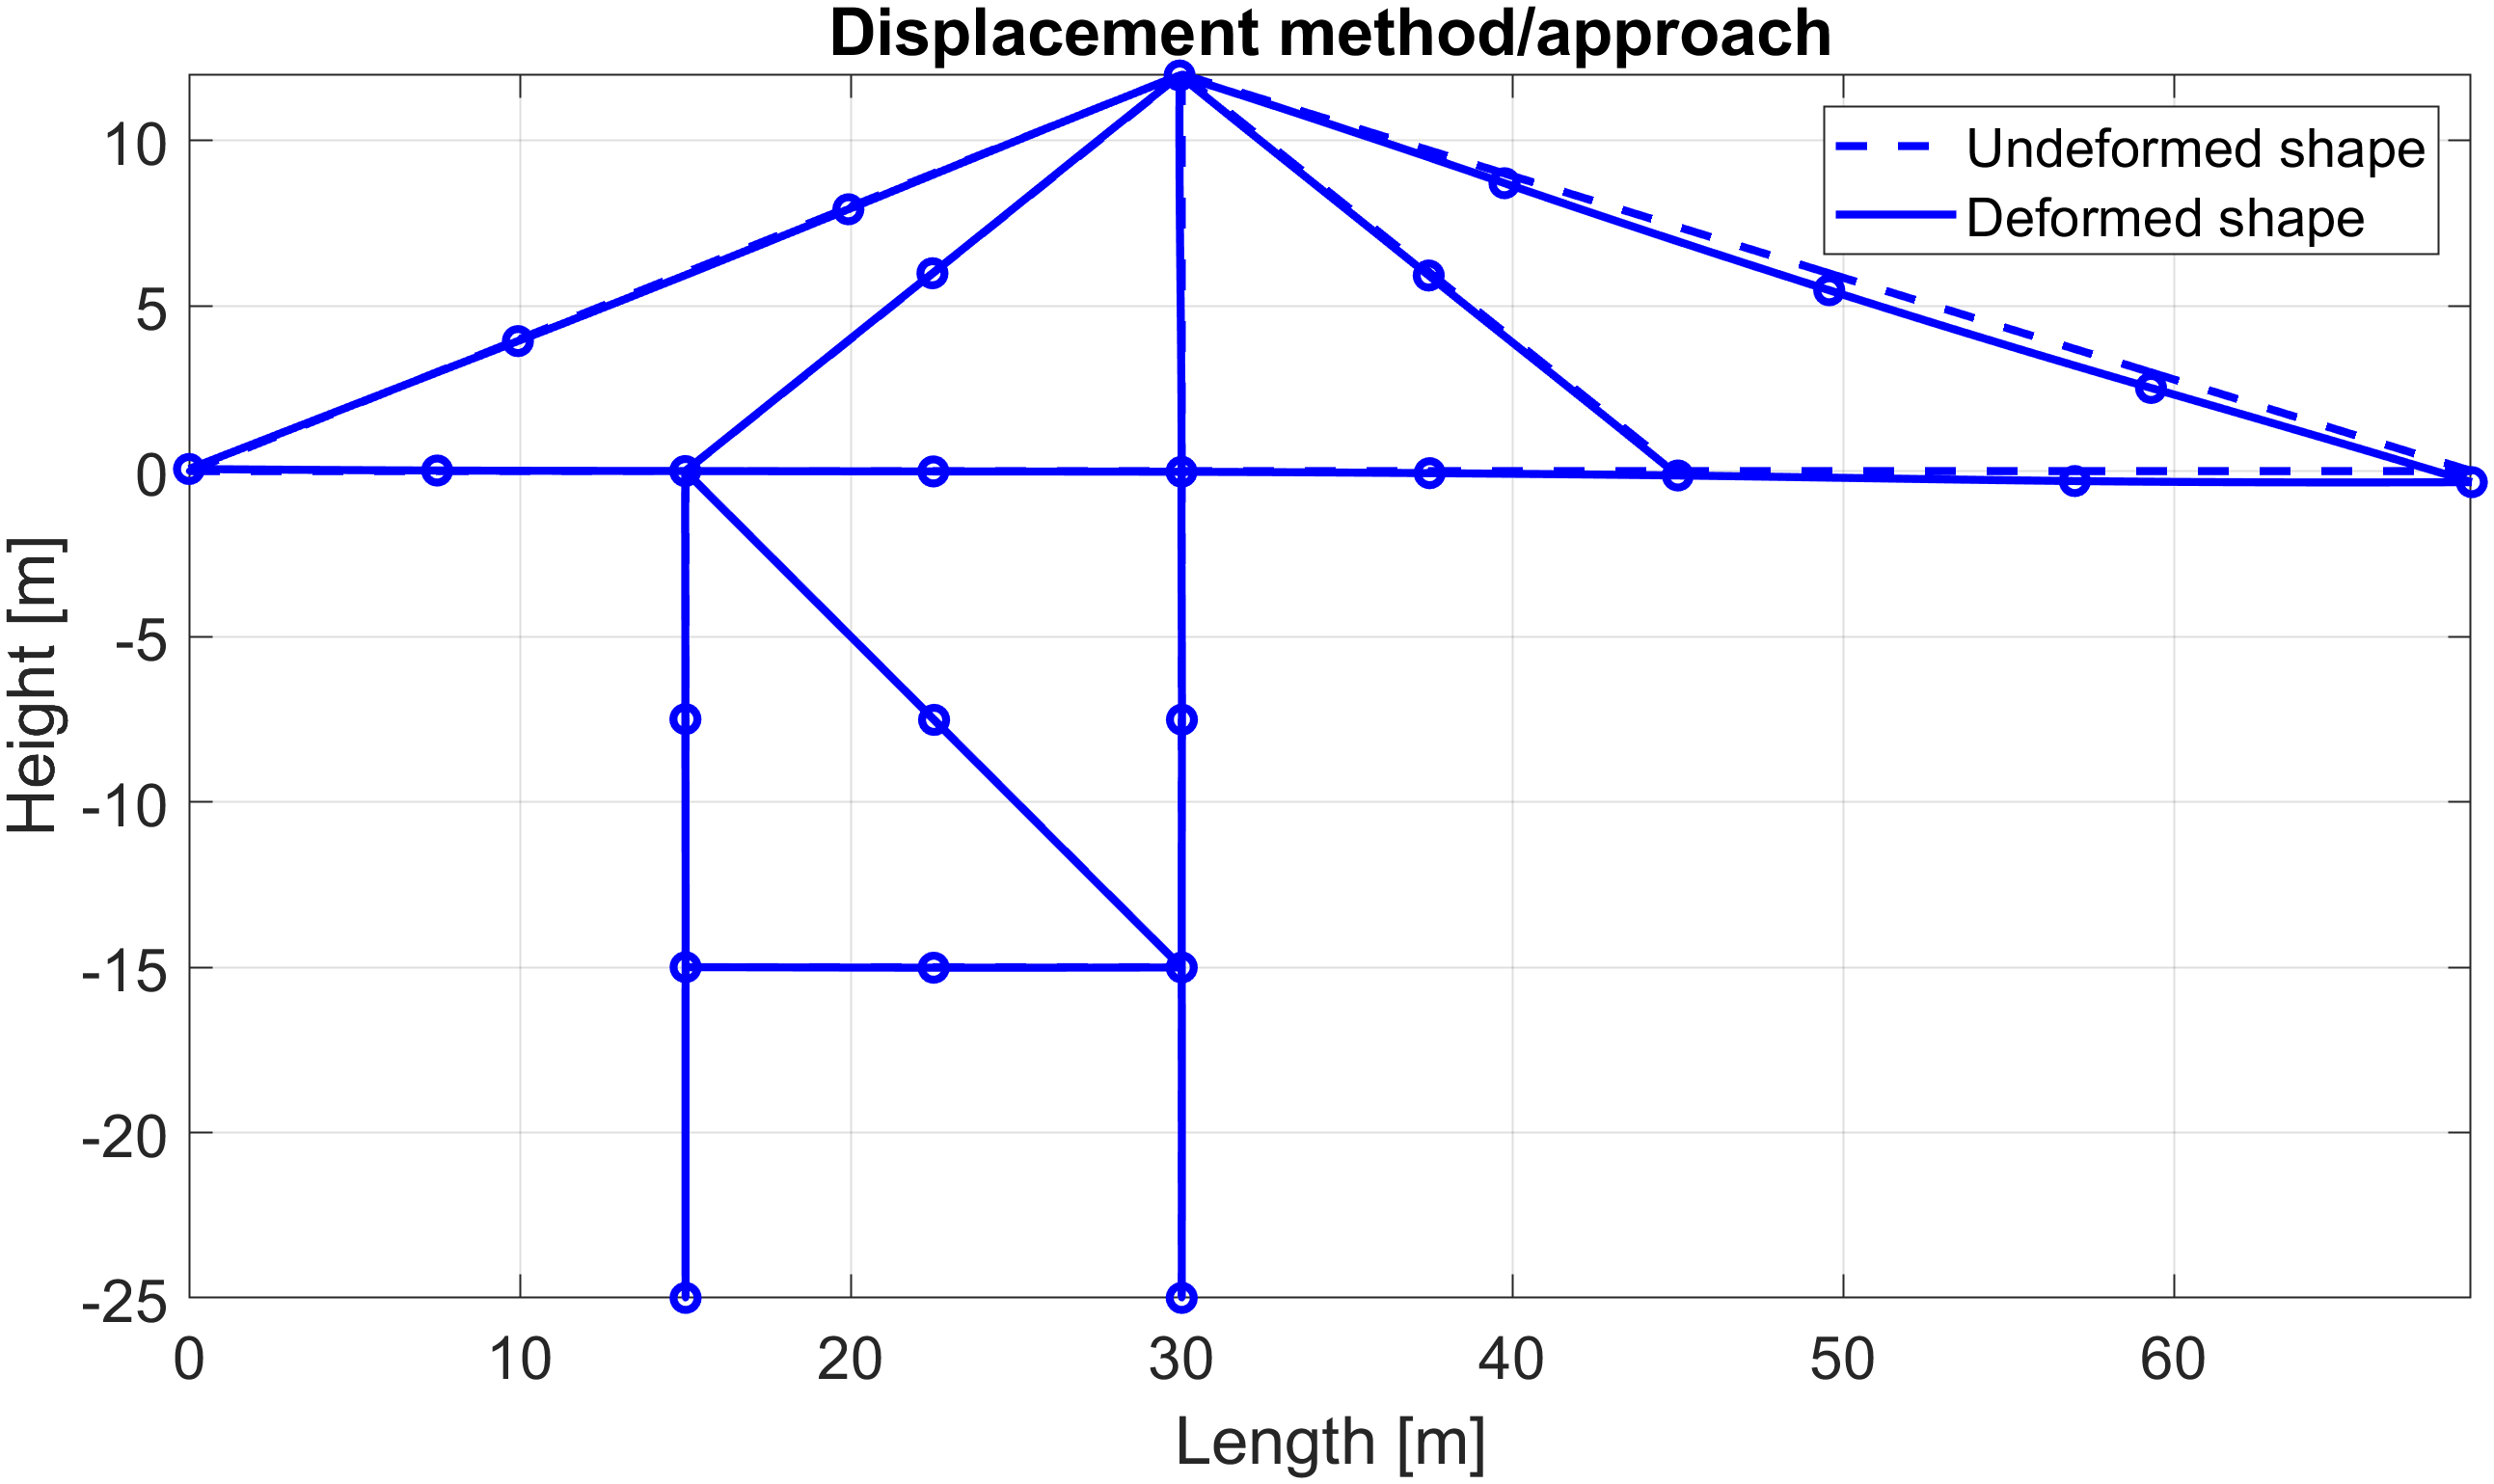
\includegraphics[width=0.45\textwidth]{img/MATLAB/Responses/Gravity_displacement.png}
    \hfill
    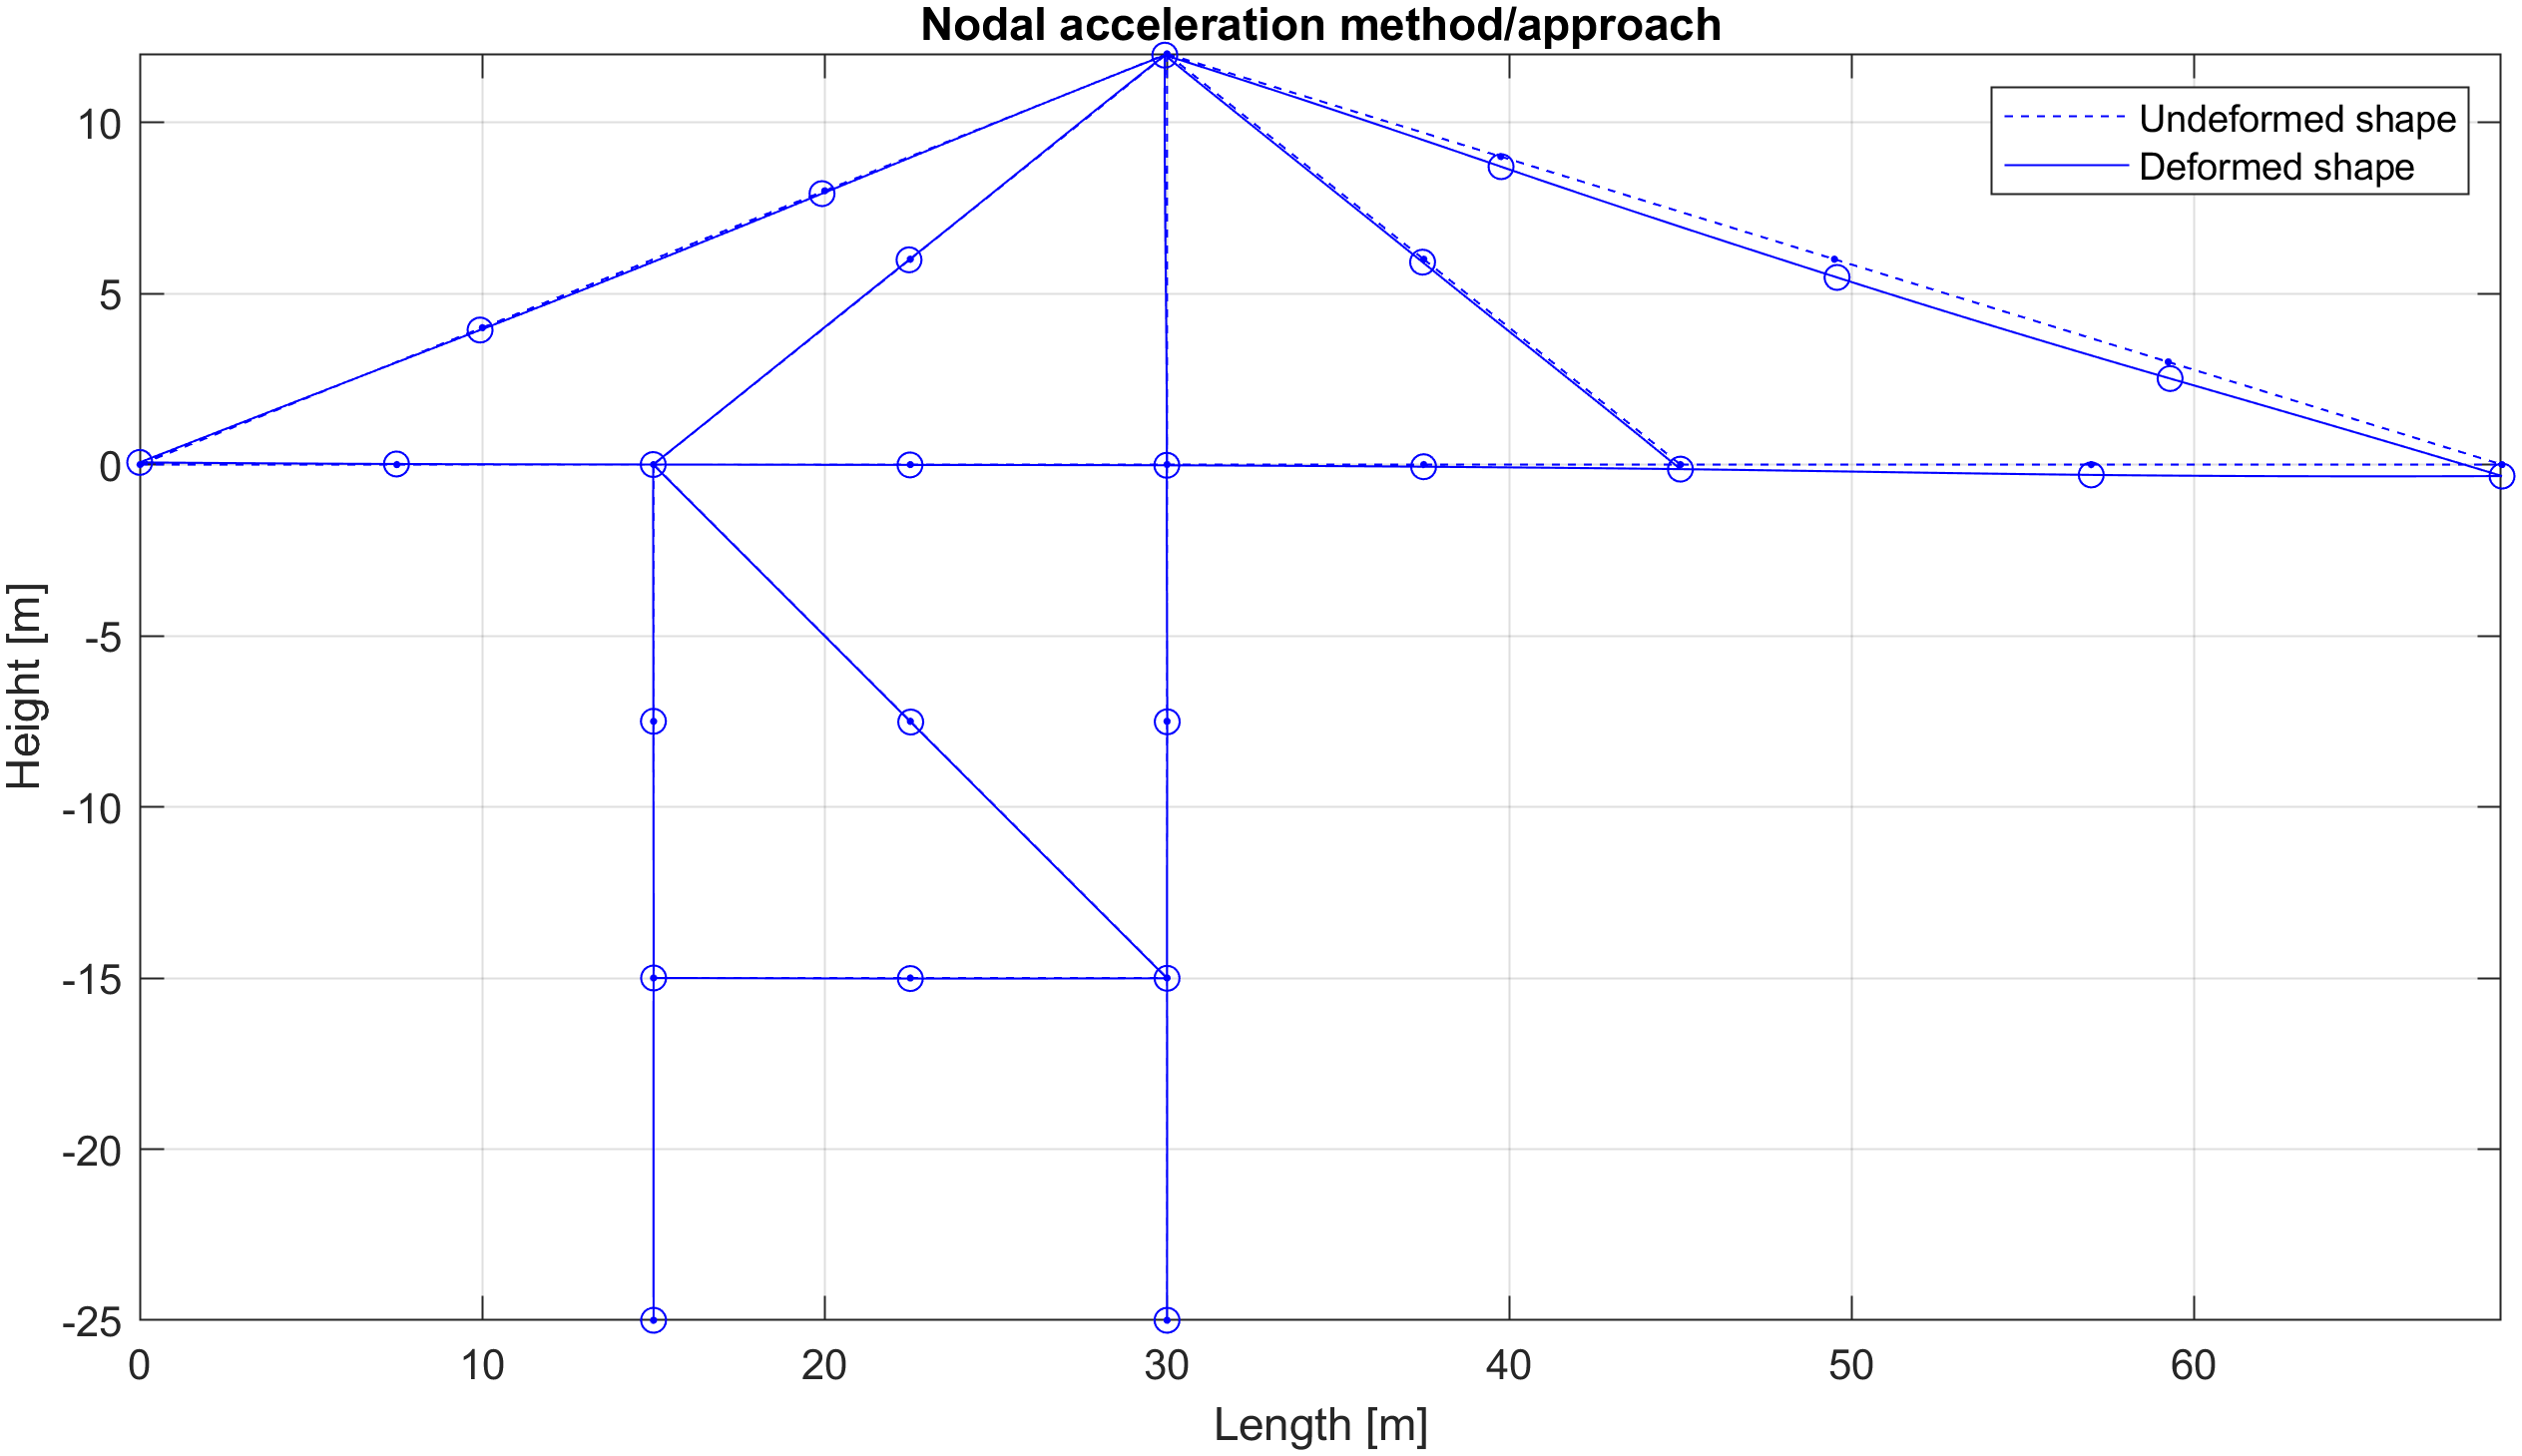
\includegraphics[width=0.45\textwidth]{img/MATLAB/Responses/Gravity_acceleration.png}
    \caption{Comparison of the static responses of the structure computed using the displacement approach and the acceleration approach.}
    \label{fig:static_responses}
\end{figure}